\documentclass[12pt]{article}

%required for setting the margin
\usepackage[paperwidth=8.5in, paperheight=11in, margin=1in]{geometry}

%required for double spacing
\usepackage{fullpage, setspace}

%sets the font to Times New Roman
\usepackage{times}

%required for setting header/footer
\usepackage{fancyhdr}
\pagestyle{fancy}

\usepackage{graphicx}
\usepackage{float}

%used for code listings
\usepackage[procnames]{listings}
\usepackage{color}

\usepackage[hyphens]{url}
\usepackage[hidelinks]{hyperref}

\usepackage{longtable}

%used for adding dots to the table of contents
\usepackage{tocloft}
\renewcommand{\cftsecleader}{\cftdotfill{\cftdotsep}}

\setlength{\parskip}{0.2cm}

\lhead{NDT MCL ROS Node Documentation}
\chead{}
\rhead{}

%we clear the center footer, where the page number is initially displayed
\lfoot{Thoduka and Mitrevski}
\cfoot{}
\rfoot{\thepage}

%we set spacing between the header and the body of the document
\setlength{\headsep}{0.2in}

%we hide the line that is displayed below the header by default
\renewcommand{\headrulewidth}{0.4pt}
\renewcommand{\footrulewidth}{0.4pt}
\renewcommand{\UrlFont}{\normalsize}

\begin{document}
	\definecolor{keywords}{RGB}{0,0,255}
	\definecolor{comments}{RGB}{0,100,0}
	\definecolor{purple}{RGB}{100,0,200}
	\definecolor{black}{RGB}{0,0,0}
	\definecolor{gray}{RGB}{230,230,230}

	\begin{titlepage}
		\vspace*{\fill}
		\begin{center}
			\begin{spacing}{1.5}
				NDT MCL ROS Node Documentation
				\linebreak
				Santosh Thoduka and Aleksandar Mitrevski
				\linebreak
				Bonn-Rhein-Sieg University of Applied Science
				\linebreak \linebreak
				June 19, 2014
			\end{spacing}
		\end{center}
		\vspace*{\fill}
	\end{titlepage}

\setcounter{page}{2}

\newpage
	\setlength{\parindent}{0.0in}

	%we center the table of contents title
	\renewcommand*\contentsname{\hfill Contents \hfill}
	\tableofcontents

\newpage

	\section{Introduction}
	\label{sec:introduction}

	The NDT-MCL (Normal distribution transform Monte Carlo localisation) ROS node is an implementation of the NDT-MCL algorithm for localisation against an NDT map. This document makes an attempt at introducing the node, including implementation and usage details, in a manner that improves the presentation provided by [4]. In order to do that, the rest of the document includes a brief introduction to NDT-MCL in section \ref{sec:ndtMclIntroduction}, a description of the node in section \ref{sec:nodeDescription}, our modifications in section \ref{sec:implementedModifications}, some usage details in section \ref{sec:usage}, remaining issues in section \ref{sec:remainingIssues}, as well as suggestions for potential improvements and modifications in section \ref{sec:potentialImprovements}.

	\section{Target Audience}
	\label{sec:targetAudience}

	This document intends to provide an overview of the NDT-MCL ROS node, focusing not only on its usage, but also on certain internal implementation details. As a result, it might be useful for developers who need to work with, modify, or maintain the node, but also for developers who are developing similar nodes and need an orientation about the complexity of such a development effort.

	Ideally, the document will be updated as the node is modified and improved. Its ultimate goal is being a constantly updated development documentation where developers can find all the necessary details regarding the NDT-MCL node.

	\section{NDT MCL - A Short Introduction}
	\label{sec:ndtMclIntroduction}

	Normal distribution transform Monte Carlo localisation (NDT-MCL), described in [1], is a localisation algorithm whose goal is providing a close and consistent estimate to the true position of a robot in a given environment. NDT-MCL uses a discretised, grid-based, representation of an environment; however, unlike other localisation algorithms, which use occupancy grids to represent a map, NDT-MCL parameterises grid cells by Gaussian distributions, employing a so-called NDT representation as suggested by [2].

	Given that the algorithm is an instance of the Monte Carlo family, the localisation steps remain the same as in grid-based localisation: calculating a pose likelihood, updating particle weights, and resampling particles. The only difference in NDT-MCL is the likelihood calculation, such that $L2$-likelihood is used to express the discrepancy between the estimated and the actual robot pose.

	\section{Node Description}
	\label{sec:nodeDescription}

	The main activity of the NDT-MCL node consists of processing laser scans in a callback function, called due to the node's subscription to a laser scan topic, and updating the estimated pose of a robot based on the scans and the robot's motion. A UML diagram of the node and some background code that implements a particle filter is shown in the figure below:
	\begin{figure}[H]
		\center
		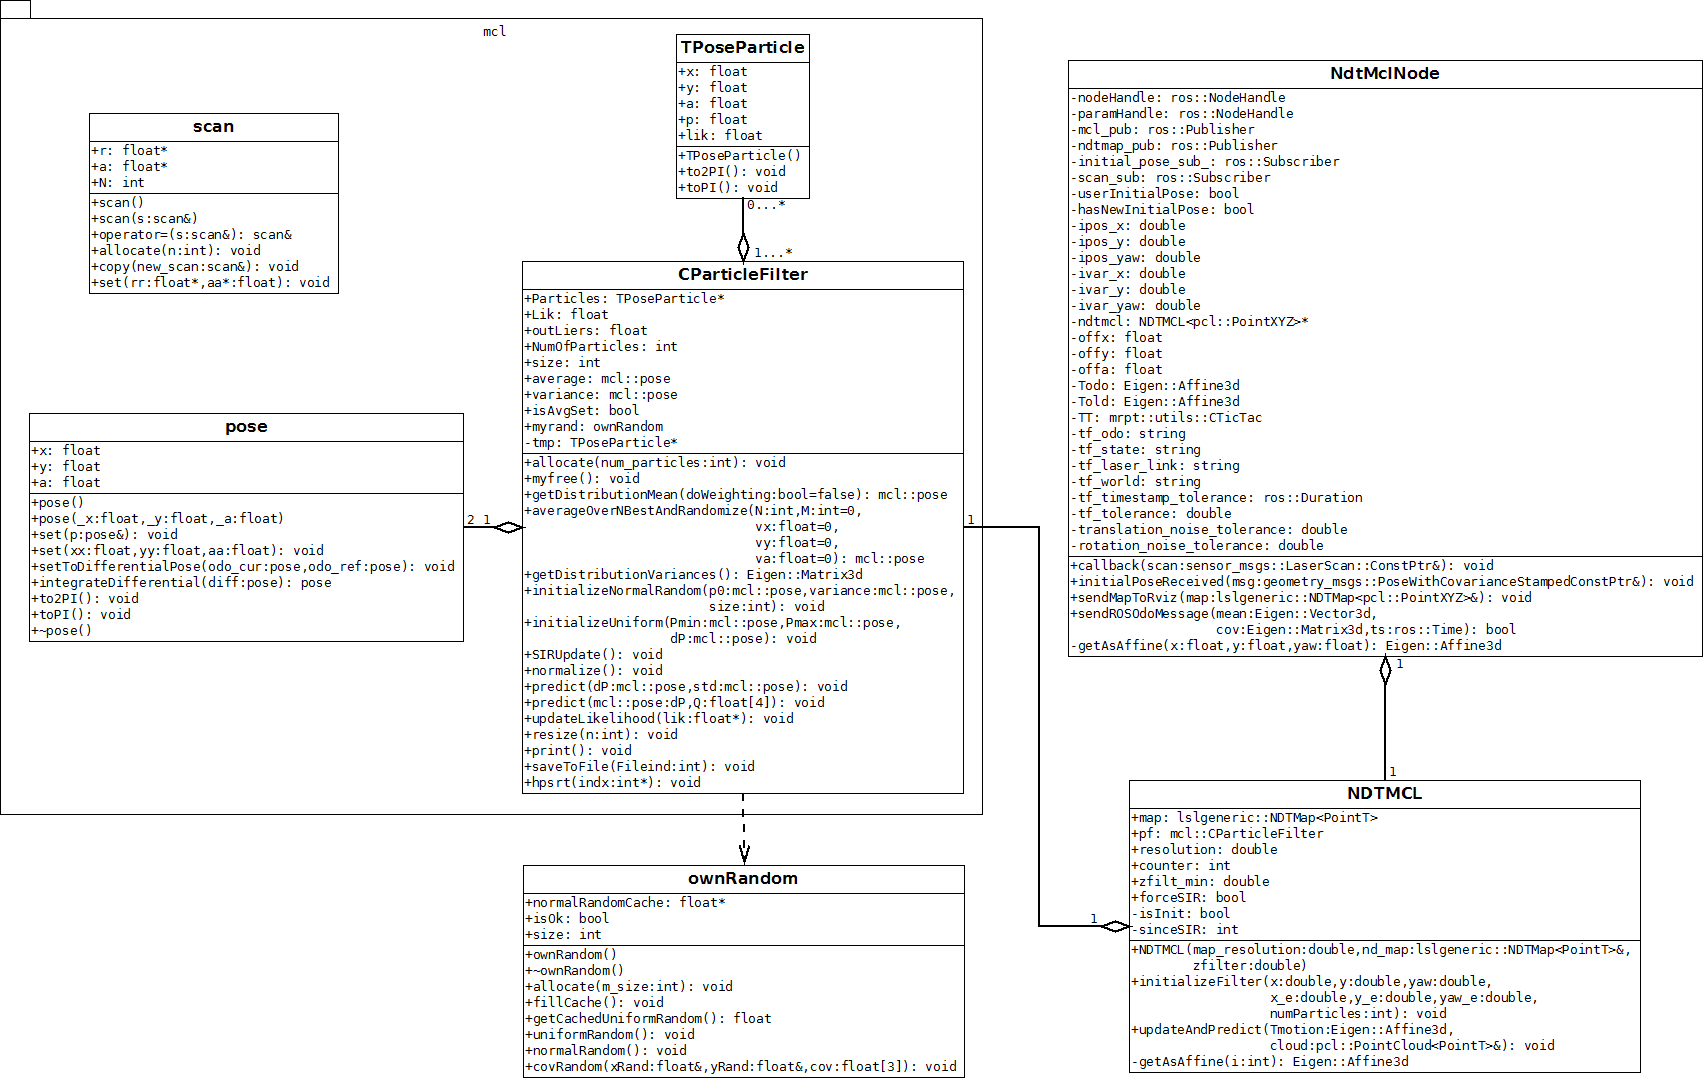
\includegraphics[width=160mm]{ndtmcl.png}
		\caption{UML diagram of the NDT-MCL node and its dependencies}
		\label{fig:umlDiagram}
	\end{figure}

	\section{Implemented Modifications}
	\label{sec:implementedModifications}

	The following list of modifications represents our contribution to the node's code:

	\begin{itemize}
		\item As can be seen in figure \ref{fig:umlDiagram}, the node is implemented as a class; this represents a modification of the initial code, which was an unstructured collection of functions and global variables.
		\item The initial implementation of the node was using a ground truth estimate of the robot's position and the localisation pose estimate was published with respect to the ground truth. The modified version of the node uses the same principle as [6], such that the published pose estimate represents a transform between the localisation frame and a robot's odometry frame.
		\item Some parameters were added to the launch file used for initialising the node; more details about these parameters are given in the following section.
	\end{itemize}

	\section{Usage}
	\label{sec:usage}

	Using the improved NDT-MCL node requires:
	\begin{itemize}
		\item An NDT map of the environment where a robot should be localised; such a map can be developed using the NDT Fuser ROS node. An explanation of NDT Fuser is beyond the scope of this document, but a sufficiently good explanation of the map creation process is given in [3].
		\item A launch file that will start the localisation node.
	\end{itemize}
	An example launch file used for initialising the NDT-MCL node is given below; some of these parameters were also used while working with our robot:
	\lstset{basicstyle=\ttfamily\footnotesize, 
	        keywordstyle=\color{keywords},
	        commentstyle=\color{comments},
		  backgroundcolor=\color{gray},
		  frame = lines,
	        stringstyle=\color{purple},
	        showstringspaces=false,
	        identifierstyle=\color{black},
	        procnamekeys={def class},
		 caption={A launch file for initialising NDT-MCL}}
	\lstinputlisting{ndtmcl.xml}
	Some of the parameters in the launch file were already present in the original implementation of the node, while others were added additionally in order to increase the node's customisation. For completeness, the following table lists all parameters that can be set through the launch file, a short description of them, and their default values. The parameters that have a * next to their name are those that were included additionally:
	%\begin{table}[H]
	%	\caption{Parameters used by the NDT-MCL node}
	%	\centering
		\begin{longtable}{| p{4.7cm} | p{7.2cm} | p{3.3cm} |}
			\caption{Parameters used by the NDT-MCL node} \\\hline
			{\bf Parameter name} & {\bf Description} & {\bf Default value} \\\hline
			{\it input\_laser\_topic} & Name of the topic where laser scans are published & {\it /base\_scan} \\\hline
			{\it tf\_base\_link} & Name of a robot's base link frame & {\it /base\_link} \\\hline
			{\it tf\_laser\_link} & Name of a laser frame; the frame should be expressed in terms of the base link frame & {\it /hokuyo1\_link} \\\hline
			{\it tf\_odom*} & Name of the robot's odometry frame & {\it odom} \\\hline
			{\it tf\_world*} & Name of the localisation frame & {\it map} \\\hline
			{\it tf\_timestamp\_tolerance*} & A number describing a discrepancy between the times when a transform is published and requested & {\it 1.0} \\\hline
			{\it translation\_noise\_tolerance*} & Translation noise tolerance (in meters) used for deciding whether a robot has really moved & 0.01 \\\hline
			{\it rotation\_noise\_tolerance*} & Rotation noise tolerance (angle in degrees) used for deciding whether a robot has really rotated & 0.5 \\\hline
			{\it sensor\_pose\_x} & X coordinate of a laser with respect to the base frame & {\it 0.0} \\\hline
			{\it sensor\_pose\_y} & Y coordinate of a laser with respect to the base frame & {\it 0.0} \\\hline
			{\it sensor\_pose\_th} & Rotation angle of a laser with respect to the base frame & {\it 0.0} \\\hline
			{\it load\_map\_from\_file} & A boolean value indicating whether to load an environment map from a file & {\it false} \\\hline
			{\it map\_file\_name} & Name of a .jff file containing an NDT map; used if {\it load\_map\_from\_file} is set to {\it true} & {\it basement.ndmap} \\\hline
			{\it forceSIR} & A boolean value indicating whether to resample particles at each iteration & {\it false} \\\hline
			{\it set\_initial\_pose} & Indicates whether an initial pose is available and should be assigned & {\it true} \\\hline
			{\it initial\_pose\_x} & X coordinate of an initial pose & {\it 0.0} \\\hline
			{\it initial\_pose\_y} & Y coordinate of an initial pose & {\it 0.0} \\\hline
			{\it initial\_pose\_yaw} & Rotation angle of an initial pose & {\it 0.0} \\\hline
			{\it map\_resolution} & Resolution of the map (in meters) in which a robot is going to be localised & {\it 0.2} \\\hline
		\end{longtable}
	%\end{table}

	In order to work with a complete navigation system, the navigation of the robot should be adapted to the NDT representation used by an environment's map.
	
	\section{Remaining Issues}
	\label{sec:remainingIssues}
	
	The following are some of the issues that remain unsolved in our testing of NDT Fuser and NDT-MCL nodes:
	\begin{itemize}
		\item \textbf{Poor localisation during mapping using the NDT Fuser node}\\
		The localisation errors seem to get large when the robot is rotated. If pure translation is used while mapping, localisation is relatively good. This occurs both in simulation and in a real environment. The cause for this has not been investigated.
		\item \textbf{Incorrect pose estimation while robot is stationary}\\
		On some runs, if the robot moves around the environment and then stops, the estimated pose of the robot continues moving. Since it does not happen on every run, it is suspected this has to do with the noise related to the motion model and the translational and rotational noise tolerance. Currently, this is the most pressing issue.
		\item \textbf{Pose estimate ``jumps''}\\
		On one run, the pose estimate of the robot ``jumped'' back to the initial position of the robot after it had moved roughly 5 meters away from the initial position. This behaviour was not reproducible on subsequent runs.
		\item \textbf{Incorrect visualization of odometry}\\
		Although it is irrelevant to the functionality of the algorithm, it was noted that the odometry on MRPT visualizer is offset from the actual position of the robot by a fixed amount.	
	\end{itemize}  
	As mentioned in section \ref{sec:potentialImprovements}, adding more configuration parameters could narrow down the cause of the issues and allow faster testing.
	
	\section{Potential Improvements and Future Work}
	\label{sec:potentialImprovements}
	
	In addition to investigating and fixing the issues mentioned in section \ref{sec:remainingIssues} there are a number of improvements to the that would make testing and implementation on different platforms easier. Once the issues and improvements have been sorted out, using the NDT-based map for navigation would be the next step. 
	
	\begin{itemize}		
		\item \textbf{Better customizability}\\
		Additional configuration constants such as motion model parameters, particle filter parameters and laser model parameters can be exposed to the user through the launch file. This will allow the user to customize the node to better fit their platform and environment without modifications to the code.
		\item \textbf{Determination of map resolution from file}\\
		Currently, the map resolution needs to be specified in the launch file for both the NDT Fuser and NDT-MCL nodes and they need to match in order for the map to be usable by the NDT-MCL node. Mismatched resolutions can be avoided if the resolution of the map is encoded in the map file (.jff) itself and can be read in by the node using the map. This would require changes to the ndt\_map package.
		\item \textbf{Port visualization to rviz}\\
		The possibility of visualizing the map, particles, estimated pose and odometry in rviz should be investigated. Rviz is a 3D visualization tool for ROS and is already being used for purposes such as sending navigation goals, viewing point clouds, cost maps etc. It would be useful to integrate the visualization for NDT-MCL into the same interface.
		\item \textbf{Investigate compatibility with navigation planners}\\
	Existing ROS navigation planners such as the dwa\_local\_planner and navfn use a 2D cost map which depends on OccupancyGrid based maps [7]. In order for the NDT-based map to be used on an autonomous system, planners need to be able to use it. Hence, the use of the NDT-map with existing cost maps and planners needs to be investigated or ones that exploit the unique representation of the map need to be developed.
	\end{itemize}

	\section{Summary and Conclusions}
	\label{sec:summaryAndConclusions}

	The NDT-MCL (Normal distribution transform Monte Carlo localisation) ROS node is an implementation of the NDT-MCL algorithm for localisation against an NDT map. Being developed recently, the node has multiple potential areas of improvements: some of them were addressed during our four-week software development project, while others remain open.

	We hope that this documentation will be a good starting point for developers who need to work with the node, helping them to use and improve NDT-MCL effectively.

	\section{References}
	\label{sec:references}

	[1] J. Saarinen, H. Andreasson, T. Stoyanov, and A. J. Lilienthal, "Normal Distributions Transform Monte-Carlo Localization (NDT-MCL)," in {\it Intelligent Robots and Systems (IROS), 2013 IEEE/RSJ International Conference on}, Tokyo, Japan, 2013, pp. 382-389.

	\setlength{\parskip}{0.25in}

	[2] P. Biber, "The Normal Distributions Transform: A New Approach to Laser Scan Matching," in {\it Intelligent Robots and Systems, 2003. (IROS 2003). Proceedings. 2003 IEEE/RSJ International Conference on}, Las Vegas, NV, 2003, pp. 2743-2748.

	[3] T. Stoyanov. (2013). {\it Using NDT Fuser to create an NDT map} [Online]. Available: \url{http://wiki.ros.org/perception_oru/Tutorials/Using%20NDT%20Fuser%20to%20create%20an%20NDT%20map}

	[4] T. Stoyanov. (2014). {\it Running NDT-MCL examples} [Online]. Available: \url{http://wiki.ros.org/perception_oru/Tutorials/Running%20NDT-MCL%20examples}

	[5] T. Stoyanov. (2014). {\it NDM MCL source code} [Online]. Available: \url{https://github.com/tstoyanov/perception_oru-release/tree/release/hydro/ndt_mcl}

	[6] B. Gerkey. (2014). {\it AMCL source code} [Online]. Available: \url{https://github.com/ros-planning/navigation/blob/hydro-devel/amcl/src/amcl_node.cpp}
	
	[7] E Marder-Eppstein. (2014). {\it costmap\_2d Package Summary} [Online]. Available: \url{http://wiki.ros.org/costmap_2d?distro=hydro}

\end{document}